\documentclass[a4paper,11pt]{article}
\usepackage{exptech}
\usepackage{textcomp}
\usepackage{graphicx}
\usepackage{array}
\usepackage[babel=true]{csquotes}
\usepackage{url}
\usepackage{hyperref}
\usepackage{wrapfig}
\usepackage[export]{adjustbox}
\usepackage{titletoc}

\hypersetup{
  %bookmarks=true, % show bookmarks bar?
  pdftitle={Avalon - Rapport de pré-étude}, % title
  pdfnewwindow=true, % links in new window
  colorlinks=true, % false: boxed links; true: colored links
  linkcolor=black, % color of internal links (change box color with linkbordercolor)
  citecolor=cyan, % color of links to bibliography
  filecolor=cyan, % color of file links
  urlcolor=cyan % color of external links
}

\title{
  \textbf{Avalon}\\
  Rapport final
}
\markright{Avalon - Rapport final}
\author{
\begin{minipage}{0.4\textwidth}
	\begin{flushleft} \large
		\emph{Auteurs :}\\
		Alexandre \textsc{Audinot}\\
		Julien \textsc{Bouvet}\\
		Thierry \textsc{Gaugry}\\
		Nicolas \textsc{Hurman}\\
		Alexandre \textsc{Leonardi}\\
	\end{flushleft}
\end{minipage}
\begin{minipage}{0.4\textwidth}
	\begin{flushright} \large
		\emph{Encadrants :} \\
		Valérie \textsc{Gouranton}\\
		Ronan \textsc{Gaugne}\\
		Bruno \textsc{Arnaldi}\\
		Willy \textsc{Allègre}\\
		Jean-Paul  \textsc{Departe}\\
	\end{flushright}
\end{minipage}
}

\date{26 mai 2015}

\begin{document}
\maketitle
\thispagestyle{empty}
\begin{abstract}
\textbf{Avalon :} Environnement de Réalité Virtuelle pour l'apprentissage à l'utilisation d'appartements tremplin. Réalisation en 3D d'un appartement domotisé interactif utilisé dans le cadre de la rééducation des personnes handicapées.\newline

Le projet est proposé par le centre mutualiste de rééducation et de réadaptation fonctionnelles de Kerpape (plus particulièrement les ingénieurs du laboratoire électronique Willy Allègre et Jean-Paul Departe).\newline

Le modèle 3D de l'appartement nous est fourni, et notre travail consiste à réaliser un logiciel fonctionnel permettant de se déplacer dans l'appartement et implémentant les interactions avec les différents éléments de domotique, en plus de prendre en charge différents périphériques de contrôle. 
\end{abstract}

\begin{figure}[h!]
	\centering
	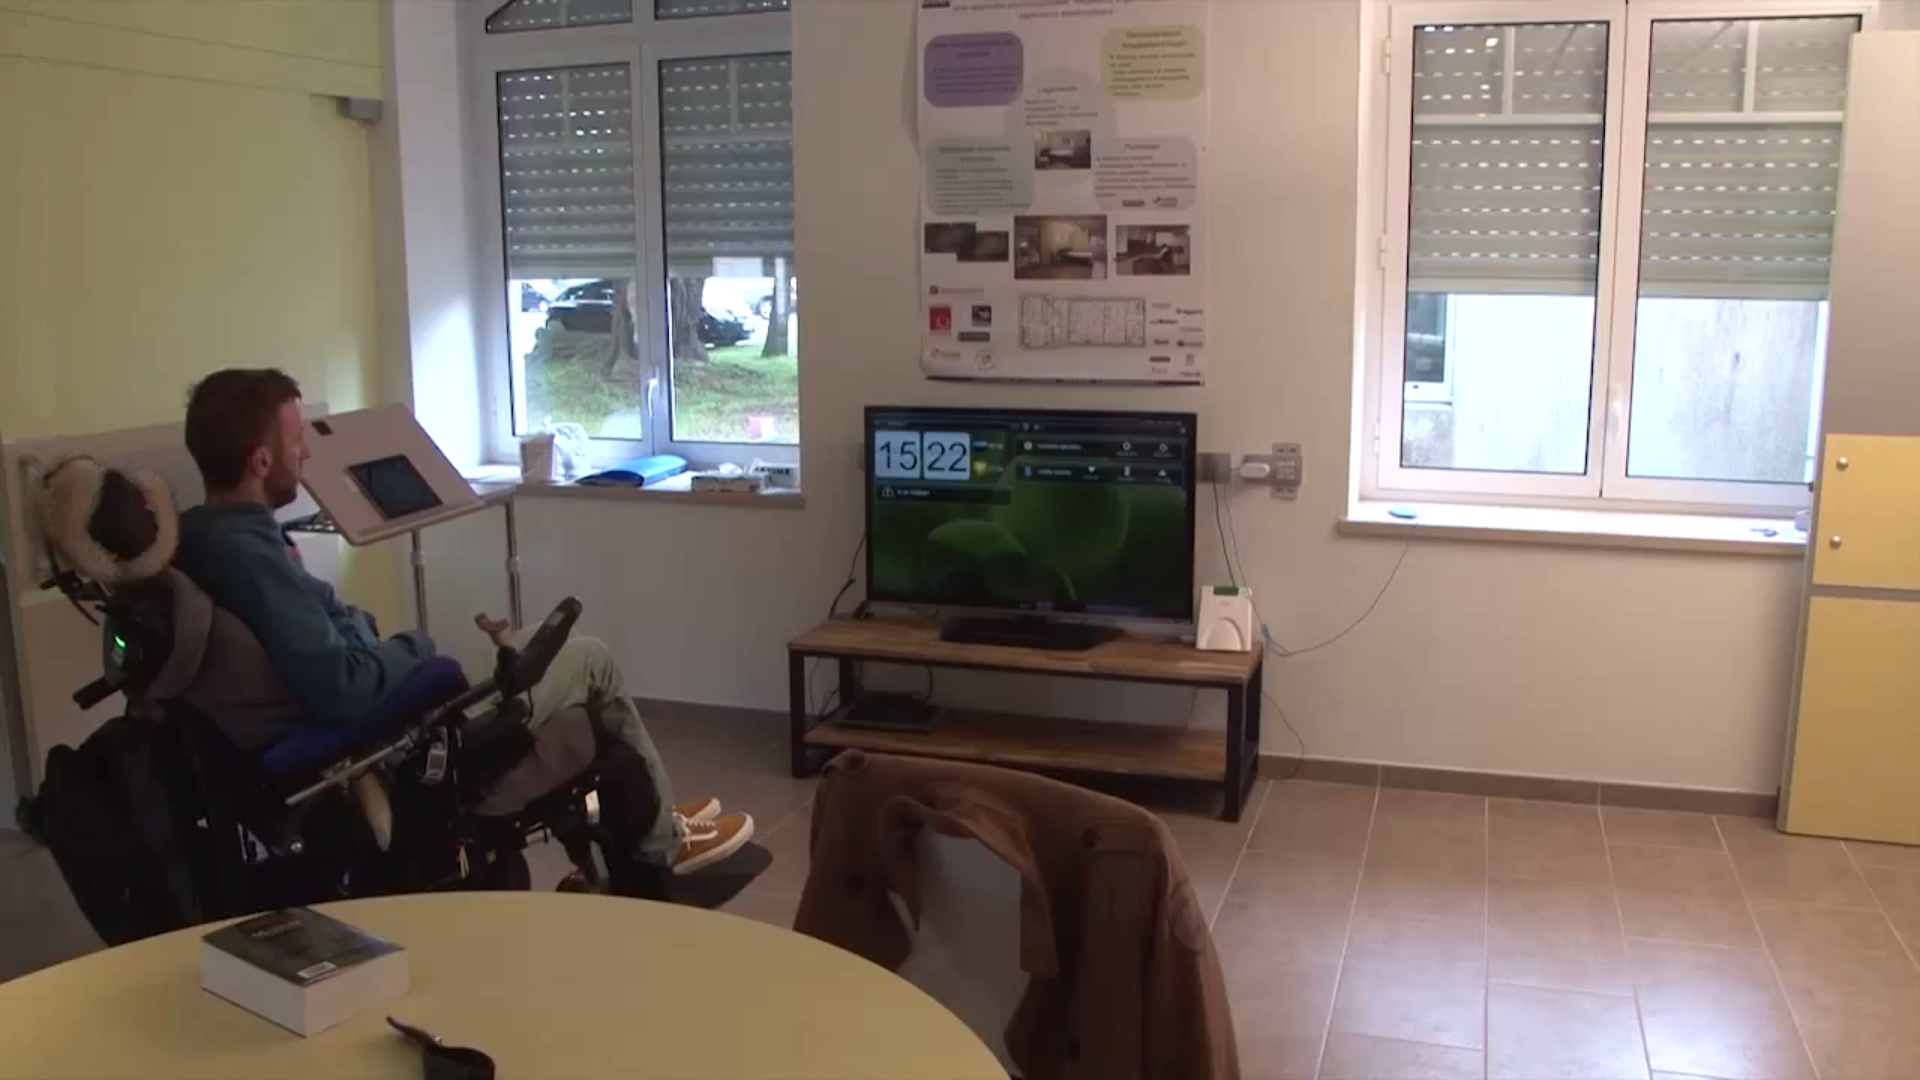
\includegraphics[width=0.7\textwidth]{8-BilanPlanification/img/screen_appart.png}
\end{figure}

%\vfill
%[width=\textwidth]
\begin{figure}[h!]
   \begin{minipage}{0.3\linewidth}
      
\includegraphics[scale=0.9]{8-BilanPlanification/img/logo_insa.jpeg}
   \end{minipage} 
   \begin{minipage}{0.2\linewidth}
      \centering
      
\includegraphics[scale=0.5,left]{8-BilanPlanification/img/logo_irisa.jpg}
   \end{minipage}\hfill
   \begin{minipage}{0.2\linewidth}
      
\includegraphics[scale=0.9]{8-BilanPlanification/img/logo_kerpape.png}
   \end{minipage}
\end{figure}

\pagebreak

\tableofcontents
\pagebreak
\section{Planification Initiale}

\subsection{Jalons}

\subsubsection{Jalons fixées par l'INSA}

Voici les dates fixées par l'INSA, qui ont fait office de jalons pendant toute la durée du projet.\\

\begin{tabular}{|l|l|}
\hline
  Date &
  Production \\
\hline
  12 février &
  Rapport de conception logicielle  \\
\hline
  2 avril &
  Page HTML  \\
\hline
  26 mai &
  Rapport Final/Annexes + Bilan Planification \\
\hline
  28 mai &
  Documentation en Ligne VF \\
\hline
\end{tabular}


\subsubsection{Jalons internes}
Dans le but de gérer notre avancement dans le temps et d'obtenir des feedback de la part de Kerpape, nous nous étions fixé des jalons \enquote{internes}.
Ceux-ci consistaient en un certain nombre de versions intermédiaires du logiciel à livrer, versions plus ou moins éloignées les unes des autres.
Nous avions fixés des niveaux de fonctionnalités pour chaque version, par exemple, la version n°3 devait intégrer les collisions dans la scène entre l'utilisateurs et les divers objets.\\

\begin{tabular}{|l|l|}
\hline
  Date &
  Production \\
\hline
  9 janvier &
  Version PC \textnumero2 \\
\hline
  9 février &
  Version PC \textnumero3 \\
\hline
  9 mars &
  Version PC \textnumero4 \\
\hline
  9 avril &
  Version PC \textnumero5 \\
\hline
\end{tabular}\\

\subsection{Méthode de travail}

Les jalons imposés, les fonctionnalités prévues en avance et les seuils d'acceptation et de validation que nous nous étions fixé nous ont naturellement conduit à travailler en suivant un cycle en V.
Les dates de rendus de rapports l'INSA ont bien sûr fait office de jalons dans ce cycle en V.
En revanche, nos jalons internes (livrables pour Kerpape) ont ajouté à ce cycle en V une coloration Agile, composée de feedback et corrections.

Un autre aspect de cette coloration agile est du refactoring régulier.
En effet, que ce soit dans les scripts ou dans les hiérarchie du projet Unity, ou encore dans l'arbre de la scène, nous avions prévu que réorganiser les fichiers, la hiérarchie des objets ou le code nous prendrai un certain temps.

\subsection{Estimations}

Pour réaliser la solution pour Kerpape nous avions fait une estimation du nombre d'heures nécessaires.
Nos estimations étaient basées sur nos expériences personnelles, venant d'autres projets, et de divers retours d'expérience.
Nous avions estimé à environ 600 heures de travail environ les fonctionnalités restantes après le mois de Février.
Dans ce planning nous avions compté les week end, les séances de projets, les vacances mais pas les semaines de partiels ni les semaines de révisions.

\subsubsection{Chronologie du projet}
Cette vue (cf.\textsc{figure~\ref{fig:timeline}}) est la plus synthétique que nous ayons réalisée, elle donne une vue d’ensemble du projet ne comprenant que les plus grandes étapes. 
\begin{figure}[h]
	\centering
	\caption{Chronologie générale}
		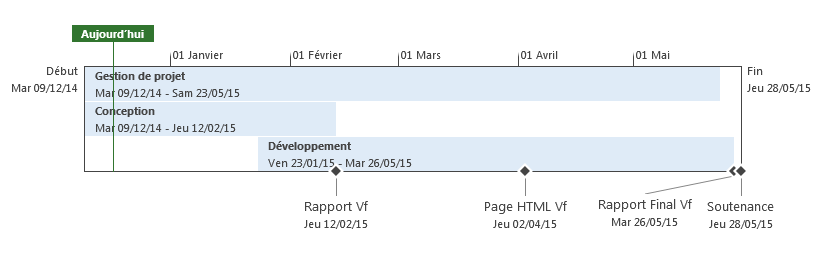
\includegraphics[width=\textwidth]{8-BilanPlanification/img/timeline.PNG}
	\label{fig:timeline}
\end{figure}

\subsubsection{Temps de travail cumulé}
Le temps de travail cumulé (cf.\textsc{figure~\ref{fig:avancement}}) restant est assez équilibré tout au long du projet avec toutefois quelques variations brusques autours des jalons précédemment définis.
Ces variations sont liées au fait que nous avons dégagé plus de temps autour des jalons en cas de problèmes.

\begin{figure}[h]
	\centering
	\caption{Temps de travail cumulé restant}
		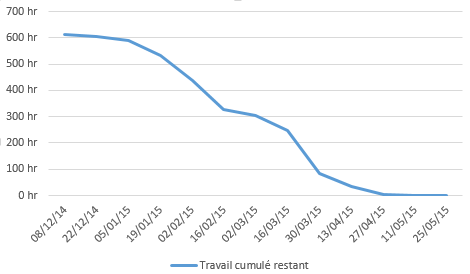
\includegraphics[width=\textwidth]{8-BilanPlanification/img/avancement.PNG}
	\label{fig:avancement}
\end{figure}
\pagebreak
\section{Evolution du projet}
\subsection{Planning}
Nous avons globalement respecté les dates limites qui nous avaient été fixées.
Malheureusement, nous avons raté de 24h la date de rendu de la page HTML, suite à une erreur d'organisation de notre part.
En effet, nous n'avions pas désigné de façon claire la personne chargée de déposer l'archive.
Suite à cet évènement, nous avons repris le schéma que nous utilisions jusque là, ie un responsable par livrable.

Par ailleurs, contrairement à ce que l'on aurait pu penser, les vacances ont été un réel problème : la plupart des tâches
de développement que nous réalisions étaient par binôme, pour améliorer la productivité étant donné la multitude
de problèmes que nous avons rencontré. Il a été compliqué de tenir compte des impératifs de chaque personne
pour arriver à un planning convenable, ce qui nous a poussé à favoriser le travail \enquote{sur place} par la suite.

Plusieurs évènements sont également venus modifier notre planning, notamment l'arrivée puis le départ d'un nouveau membre
pour lequel nous avons dû investir un peu de notre temps afin de le former.

\subsection{Versions intermédiaires}
A l'origine, nous avions prévu un large éventail de versions intermédiaires. Ayant choisi un cycle agile, cela avait du
sens car nous aurions pu les fournir à Kerpape au fur et à mesure de l'avancement du projet.

Cependant, après la seconde version intermédiaire, nous avons choisi d'arrêter de les fournir à Kerpape car les changements
visibles étaient mineurs, l'essentiel de la progression étant au niveau de l'architecture permettant au logiciel d'être
extensible. Nous avons fixé une date avec eux pour les rencontrer en personne une seconde fois, à l'IRISA, où nous
leur avons fait une démonstration du logiciel à la fois sous PC et sur la plate-forme Immersia. Willy Allègre et Jean-Paul
Despartes se sont montrés satisfaits, ce qui nous a conforté dans ce choix. Nous avons tout de même réalisé ces
versions intermédiaires en interne, pour suivre le planning établi.

\subsection{Ecarts par rapport au planning}


\subsubsection{Middle VR - Difficultés imprévues}
Nous nous sommes cependant heurtés à plusieurs problèmes au cours du projet, qui n'ont cessé de prendre de l'ampleur
avec la spécialisation de notre application vers l'interface clavier/souris. Plus nous avancions, plus MiddleVR
nous mettait des batons dans les roues. En effet, MiddleVR est prévu pour les environnements de réalité virtuelle,
où les périphériques d'entrée sont des trackers donnant directement une position et une orientation. Le logiciel
demandé par Kerpape ne rentrant pas dans cette catégorie, nous avons à plusieurs reprises dû réécrire des parties de la
logique de MiddleVR, voire même, quand c'était impossible, d'écrire des scripts annulant ce que MiddleVR faisait pour
ensuite appliquer notre propre logique (par exemple, la gestion de la caméra, les déplacements au clavier, la fonction
\enquote{focus sur un objet}).

Nous n'avions absolument pas envisagé ce lourd travail, ne connaissant pas les détails d'implémentation de MiddleVR
lors de la phase de spécification. Nous avons tout de même dû continuer à l'utiliser, à cause de la contrainte de la
diversité des plate-formes sur lesquelles le logiciel devait pouvoir s'exécuter.

\subsubsection{Multiples présentations}

Nous avons aussi eu diverses présentations à effectuer sur notre projet tout au long de l'année, ce qui a mobilisé
2 ou 3 personnes pour leur préparation et leur démonstration pendant plusieurs jours. Cela a cependant été une
bonne expérience, permettant de mettre en avant notre travail et de faire connaître les technologies que nous
utilisions.

Nous avons ainsi présenté notre projet aux 2ème années de l'INSA de Rennes, mais également lors des journées portes ouvertes, ainsi qu'à des membres de la promo INFO 1986, aux organisateurs de la BattleDev ...

\subsubsection{Risques}

Au niveau des risques, nous avions envisagé l'indisponibilité de quelques membres du groupe ou une panne de leurs
équipements informatiques, cependant dans les dernières semaines du projet, plusieurs évènements imprévus ou mal
prévus sont venus mettre à l'épreuve notre préparation : tout d'abord, juste après les partiels, sur la période que
nous avions désignée pour finir le logiciel, la connection Internet de l'INSA a été inutilisable pendant 3 jours,
rendant impossible toute avancée signiticative (pas d'accès à la documentation, pas possible de récupérer le code source,
les fichiers de démo...). Ensuite, des évènements associatifs pour lesquels une indisponibilité partielle était prévue
ont occupé à temps plein (08h->02h) les personnes concernées suite aux problèmes recontrés là-bas.

Ces deux baisses de capacité de travail ont entraîné un retard qui a été partiellement absorbé par la marge que nous
nous étions allouée, mais ont tout de même nécessité une cadence de travail accrue sur les jours restants.

\pagebreak
\section{Méthodes d'organisation \& planification}

\end{document}
